\documentclass[a4paper,12pt]{article}
\usepackage[slovene]{babel}
\usepackage[utf8]{inputenc}
\usepackage{multicol}
\usepackage{fullpage}
\usepackage{guitar}
\usepackage{titlesec}
\usepackage{graphicx}
\setcounter{secnumdepth}{-1} 
\usepackage[absolute]{textpos}
\titleformat{\chapter}{\large\bfseries}{\thesection}{1em}{}
\titleformat{\section}{\Large\bfseries}{\thesection}{1em}{}
\titleformat{\subsection}{\large\bfseries}{\thesection}{1em}{}

\begin{document}
\pagenumbering{Roman}
\begin{titlepage}
\begin{textblock*}{297mm}(-6mm,-0mm)
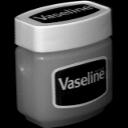
\includegraphics[width=\paperwidth]
{frontpages/obj10__64.png}\end{textblock*} \
\end{titlepage}
\setlength{\columnseprule}{0.5pt}
\begin{multicols}{2}
\tableofcontents
\end{multicols}
\pagebreak

\setlength{\columnseprule}{0.5pt}
\begin{multicols}{2}
\pagenumbering{arabic}
\section{Akordi}
\begin{guitar}
[A - X02220  Am - X02210]

[B - X13331  Bm - X13321]

[C - X32010  Cm - X35543]  

[D - XX0232  Dm - XX0231] 

[E - 022100  Em - 022000] 

[F - 133211  Fm - 133111]

[G - 320003  Gm - 355333]

[H - X24442  Hm - X24432]


[A7 - X02020  B7 - X13131]

[C7 - X32310  D7 - XX0212]

[E7 - 020100  F7 - 131211]

[G7 - 320001  H7 - X21202]


[Am7 - X02010  Bm7 - X13121]

[Cm7 - X35343  Dm7 - XX0211]

[Em7 - 022030  Fm7 - 131111]

[Gm7 - 353333  Hm7 - X24232]


[C# - X46664  D# - 779997]

[F# - 244322  G# - 466544]


[C#m - X46654  D#m - 779987]

[F#m - 133111  G#m - 466444]


[A6 - X02222  C6 - X055555]

[D6 - X077777 E6 - X099999]


[ASUS2 - X02200]

[ASUS4 - X02230]

[DSUS2 - XX0320] 

[DSUS4 - XX0233]

[ESUS4 - 022200]

[CMAJ7 - X32000]

[FMAJ7 - 103210]

[GMAJ7 - 3X0032]

[DADD4/ADD2 - 554030]

\end{guitar}
\subsection*{Barre akordi}
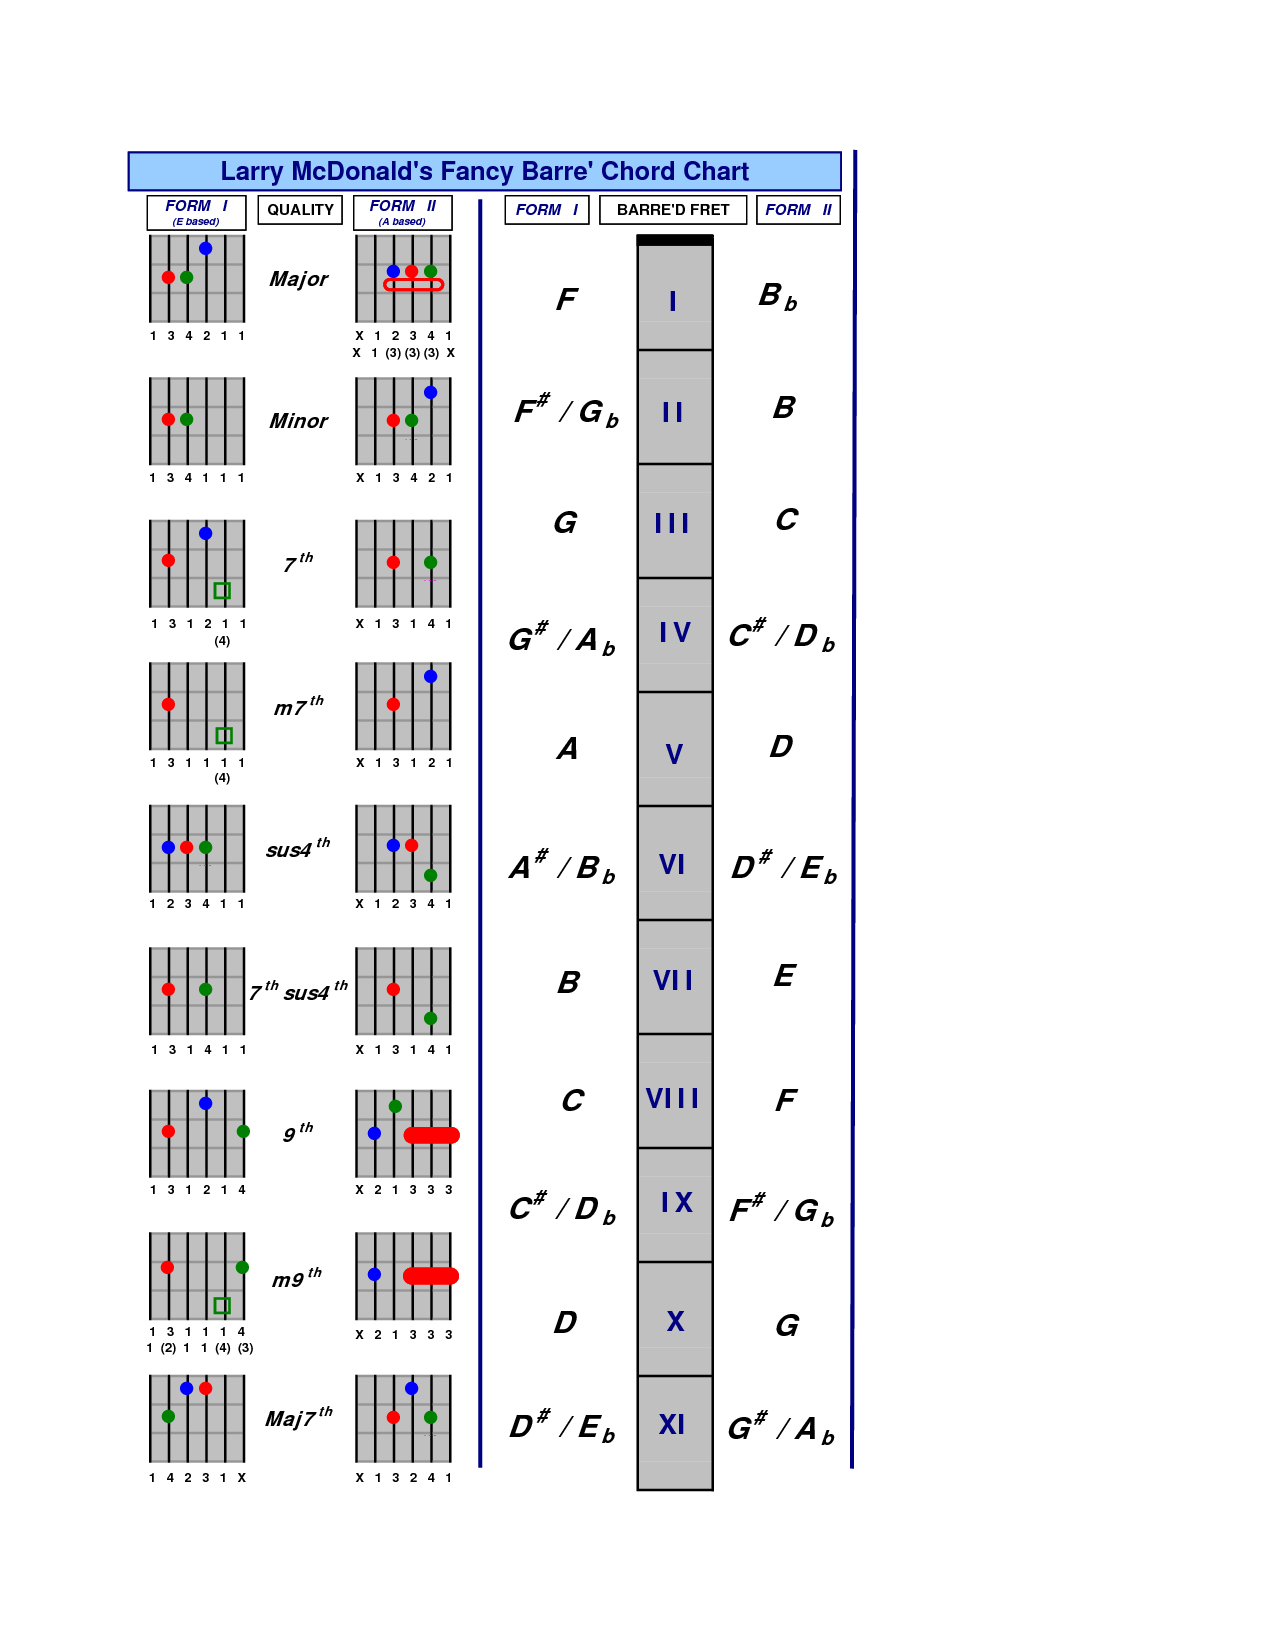
\includegraphics[width=140mm]{img/barre.png}
\clearpage
\section{Bor do bora}
\subsection*{Taborniška}
\begin{guitar}
[C]Bor do bora, jelka z [G]jelko,
kakor gora, kakor [C]jeklo.
[C]Rod do roda, vsi v dru[F]zini,
smo v svo[C]bodni [G]dom[C]ovini.


[F]Sile močne, [C]sile, sile čvrste,   
[G]strnjene so v [C]naše vrste.
[F]Sile močne, [C]sile, sile čvrste
[G]naše vrste [C]so.


Šotor dom, narava mati,
oče grom, gozdovi brati.
Od sestra planin na morje,
širi, širi se obzorje.

          
Sile močne....


Glas severa, juga pesem 
tisočera v svet ponese
taborno nam geslo pravo:
Hej taborniki v naravo!

         
Sile močne....

\end{guitar}
\end{multicols}
\clearpage
\clearpage
\null
\vfill
\center

\includegraphics[width=100px]{img/licence.png}

Pesmarica je zaščitena z licenco CC-BY-NC-SA. Vse pesmi so delo in last avtorjev. Morebitne napake in predloge sporočite na pesmarica.info@gmail.com 

Izvorna koda (LaTeX) ter PDF sta dostopna na https://github.com/gztproject/Pesmarica
\end{document}
